\documentclass{beamer}
\usetheme{Madrid}
\usecolortheme{crane}


\usepackage[utf8]{inputenc}
\usepackage{amsmath}
\usepackage{amssymb}
\usepackage{pbox}
\usepackage{subcaption}

\graphicspath{ {./images/}}

\DeclareMathOperator{\logit}{logit}


%Information to be included in the title page:
\title{Aiding Television Media Planning Through Bayesian Inference and Forecasting}
\author{Matthew Tiger}
\institute{Towson University}
\date{May 2018}


\begin{document}

\frame{\titlepage}

\frame{\tableofcontents}


\section{Introduction}

\begin{frame}
\frametitle{Problem}

\end{frame}

\begin{frame}
\frametitle{TV Advertising Buying and Selling}
\end{frame}

\begin{frame}
\frametitle{Motivating Example}
Baseball example
\end{frame}

\begin{frame}
\frametitle{Formal Statement of Problem}
\end{frame}

\begin{frame}
\frametitle{Bayesian Inference}
Baseball example
\end{frame}


\section{Data}

\begin{frame}
\frametitle{Types of Data}
\end{frame}

\begin{frame}
\frametitle{Programming Schedule}
\end{frame}

\begin{frame}
\frametitle{Forecasted Impressions}
\end{frame}

\begin{frame}
\frametitle{Audience Measurement}
\end{frame}

\begin{frame}
\frametitle{Training Data}
\end{frame}

\begin{frame}
\frametitle{Audience Size Comparison}
\begin{figure}[!h]
  \centering
  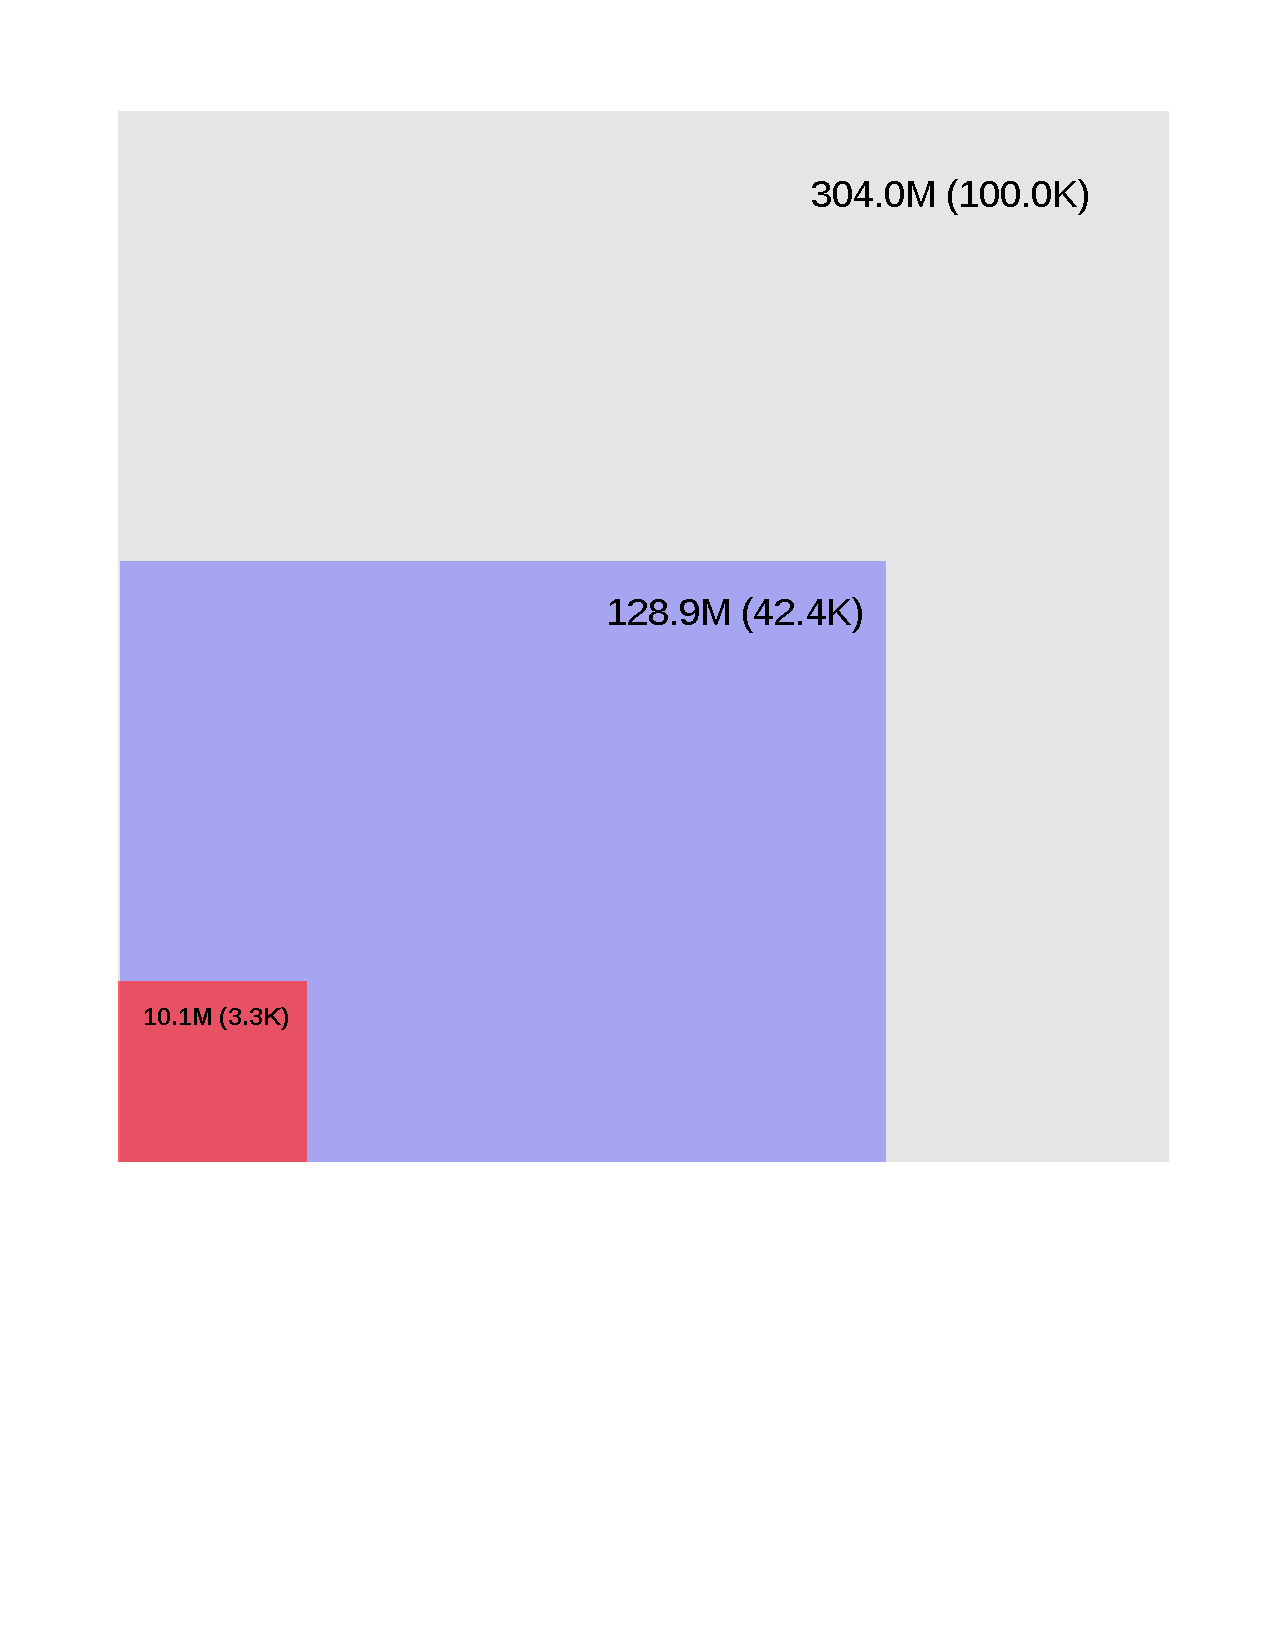
\includegraphics[scale=0.35]{panel}
\end{figure}
\end{frame}


\section{Model}

\begin{frame}
\frametitle{Units of Observation and Analysis}
\end{frame}

\begin{frame}
\frametitle{Covariates}
\begin{itemize}
  \item \emph{Time-based} covariates and \textbf{Program-based} covariates
  \pause
  \item Derived from Media Schedule
    \begin{itemize}
      \item \emph{Broadcast Month}
      \item \emph{Day of Week}
      \item \emph{Stratified Hour}
      \item \textbf{Content}
      \item \textbf{Lead-in Content}
    \end{itemize}
  \pause
  \item Derived from Audience Measurement Data
    \begin{itemize}
      \item \textbf{Genre}
      \item \textbf{Live-program}
      \item \textbf{First-run}
    \end{itemize}

\end{itemize}

\end{frame}

\begin{frame}
\frametitle{Assumptions}
\begin{itemize}
  \item We assume that the response variables $y_i$ are \emph{exchangeable} given the parameters of the model
  and the covariates of the unit of observation.

  \pause
  \item A sequence of random variable is exchangeable if the ``joint probability density $p(y_1, \dots, y_k)$ is invariant to permutations of the indexes.''
  \pause
  \item This allows us to model the data as independently and identically distributed given the covariates and unknown parameters.

\note[item]{This means the order in which the data occurs does not determine the joint probability density and therefore is unimportant.}
\end{itemize}
\end{frame}

\begin{frame}
\frametitle{Model Description}
Define model $\mathcal{M}$ to be
\begin{align*}
  y_i | X_i, n_i, \pi_i, \omega_i, \kappa_i &\sim \text{Bin}(n_i, \pi_i) \\
  \pi_i | \omega_i, \kappa_i &\sim \text{Beta}\left(\omega_i \kappa_i + 1, (1 - \omega_i) \kappa_i + 1\right) \\
  \omega_i &= \logit^{-1}\left(\beta_0 + \sum_{j=1}^{m-1}  \beta_j X_{ij}\right), \quad \beta_j \sim t_4(0, \sigma_j^2) \\&\quad \text{for $0 \leq j \leq m$}\\
  \kappa_i | X_{im} &\sim \text{Exp}(\lambda_p X_{im}), \quad \text{for $p = 0, 1$},
\end{align*}
where $\logit^{-1}(\alpha) = \frac{\exp{\alpha}}{1 + \exp{\alpha}}$.

\end{frame}

\begin{frame}
\frametitle{Model Description}
\begin{figure}[!h]
  \centering
  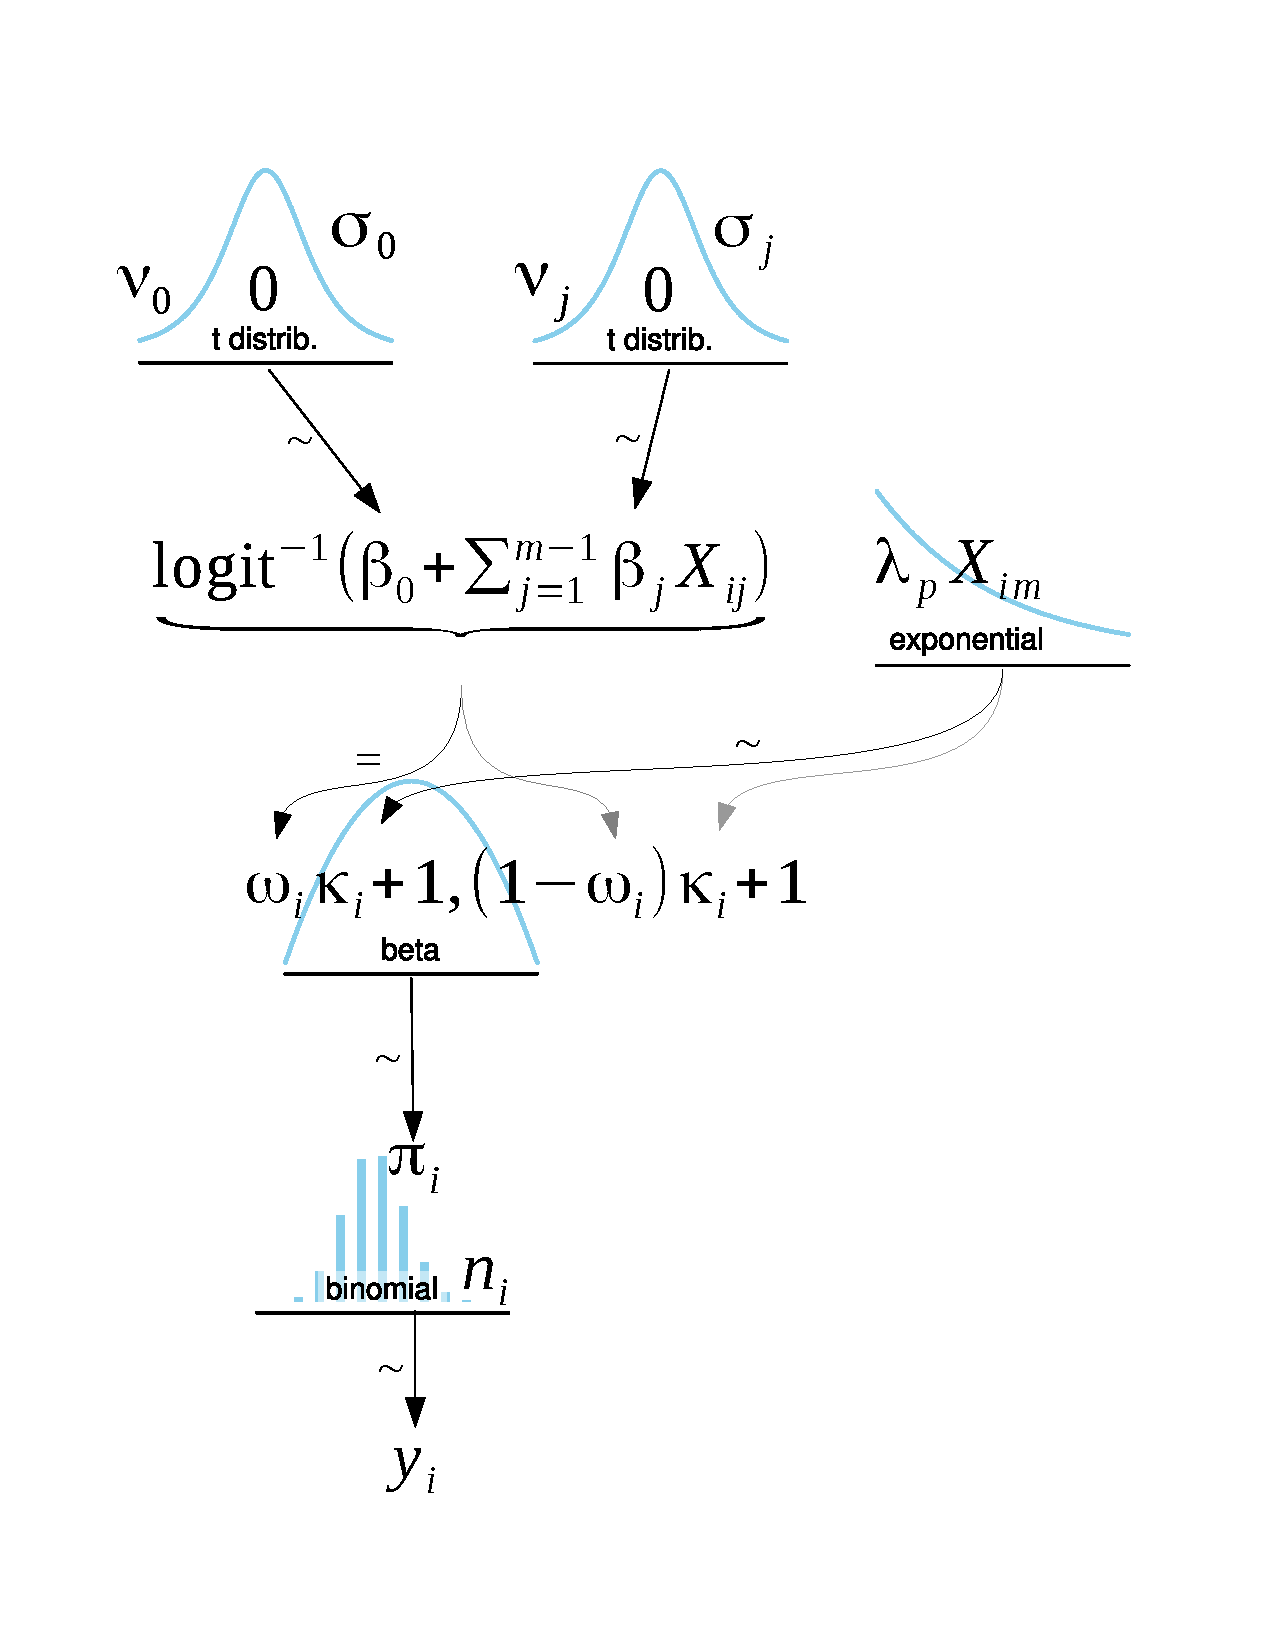
\includegraphics[scale=0.3]{kruschke_diagram}
\end{figure}
\end{frame}

\begin{frame}
\frametitle{Prior Distribution Choice}
\begin{itemize}
\item Prior distributions for coefficients $\beta_j$ and concentration parameter $\kappa_i$ are chosen to be \emph{weakly informatative}.
\pause
\item For the coefficients, this means that $\mu_j=0, \nu_j = 4$ for all $j$ and that $\sigma_j = 2.5$ if $1 \leq j \leq m$ otherwise $\sigma_0 = 5$.
\pause
\item For the concentration parameter, this means that $\lambda_p = 10^{-4}$.
\pause
  \begin{figure}[h!]
    \begin{center}
      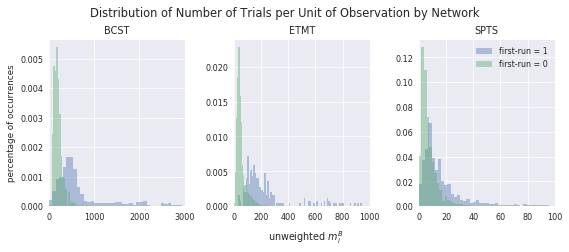
\includegraphics[scale=0.4]{kappa_explanation}
    \end{center}
  \end{figure}

\note[item]{Weakly informative here means that the priors are ``intentionally weaker than whatever prior
knowledge is available'' and act as constraints on the possible parameters that are to be sampled.}
\note[item]{This means $\beta_1, \dots, \beta_m$ are between -5 and 5 which on the logit scale are roughly 0.01 and 0.99
which is a larger effect than is to be expected by a single coefficient. We use weaker prior on intercept since more information
is available about intercept through data. Mean 0 is chosen because apriori we don't know if coefficient will be positive or negative.
}
\note[item]{Panel size is $10^5$ so $\lambda_p = 10^{-4}$ allows for parameter to be equal to total number of panelists.}
\end{itemize}
\end{frame}


\begin{frame}
\frametitle{Computation}
\begin{itemize}
\item Inference was computed using pymc3, a probabilistic programming language and library for Python.
\pause
\item The library is powered by the No U-Turn Sampler (NUTS) which is a variant of Hamiltonian Monte Carlo (HMC).
\pause
\item Parameters used for sampling:
  \begin{itemize}
    \item \texttt{target\_accept}: 0.95
    \item tuned samples: 3000
    \item drawn samples: 500
    \item number of chains: 4
  \end{itemize}
\end{itemize}
\end{frame}

\begin{frame}
\frametitle{Convergence}

\begin{itemize}
\item Approximate convergence to posterior distribution is measured through the \emph{Gelman-Rubin} statistic, denoted by $\hat{R}$.
\pause
\item Another convergence check is the number of effective samples produced by the simulation, denoted by $\hat{n_{\text{eff}}}$.
\pause
\item If $\hat{R}$ is close to 1 then we may assume we have approximate convergence. Further it is recommended that $\hat{n_{\text{eff}}} \geq 10 M$ where $M$ is the number of sampled Markov chains for all model parameters.
\pause
\item For each network model, we have that $0.99 \leq \hat{R} \leq 1.01$ and $\hat{n_{\text{eff}}} > 400$
    for all model parameters.

\note[item]{This is a measure of the between-sequence and within-sequence variance
  across the Markov chains and is used to determine if stationarity and mixing has been achieved.}
\note[item]{Number of effective samples is measured through the autocorrelation of the Markov Chain at lag $t$. More autocorrelation means less effective samples.}
\end{itemize}
\end{frame}


\section{Model Fit}

\begin{frame}
\frametitle{Posterior Predictive Checks}
\begin{itemize}
  \item ``If the model fits, then replicated data under the model should look similar
  to observed data.''
  \pause
  \item Generating data using the posterior density and checking some aspect of the generated data set is called a
    \emph{posterior predictive check}.
\end{itemize}
\pause
Let $y$ be the observed data and $\theta$ be the vector of model parameters. Define $y^{\text{rep}}$ to be the replicated data
that could have been generated given $\theta$, i.e.\

\begin{align}\label{form:yrep}
    p(y^{\text{rep}} | y) = \int p(y^{\text{rep}}|\theta)p(\theta | y) d\theta.
\end{align}
\note[item]{Note the replicated data is dependent on the data. This formula marginalizes out the vector of parameters.}
\end{frame}

\begin{frame}
\frametitle{Replicated versus Actual Data}
\begin{figure}
  \begin{subfigure}{.75\textwidth}
    \centering
    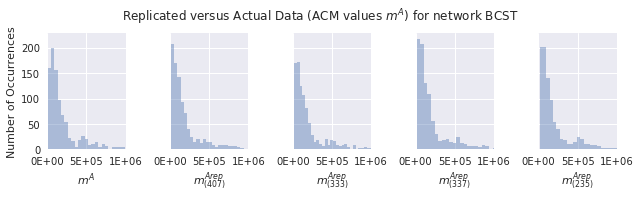
\includegraphics[scale=0.35]{BCST_m_rep}
  \end{subfigure}
  \begin{subfigure}{.75\textwidth}
    \centering
    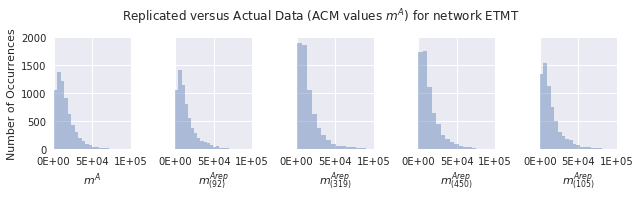
\includegraphics[scale=0.35]{ETMT_m_rep}
  \end{subfigure}
  \begin{subfigure}{.75\textwidth}
    \centering
    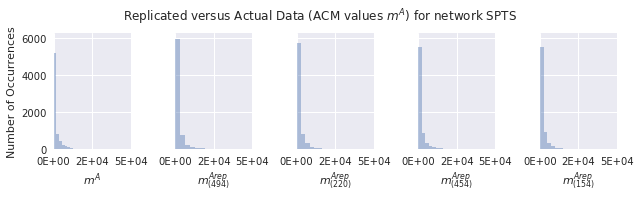
\includegraphics[scale=0.35]{SPTS_m_rep}
  \end{subfigure}
\end{figure}
\end{frame}

\begin{frame}
\frametitle{Replicated versus Actual Data}
    \begin{figure}[!h]
      \begin{subfigure}[b]{.75\textwidth}
        \centering
        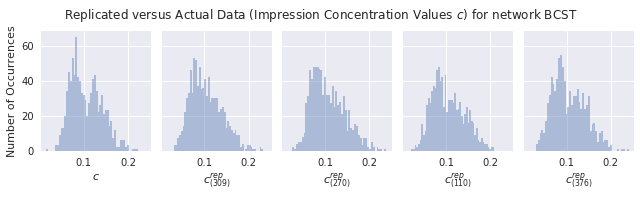
\includegraphics[scale=0.35]{BCST_c_rep}
      \end{subfigure}
      \begin{subfigure}[b]{.75\textwidth}
        \centering
        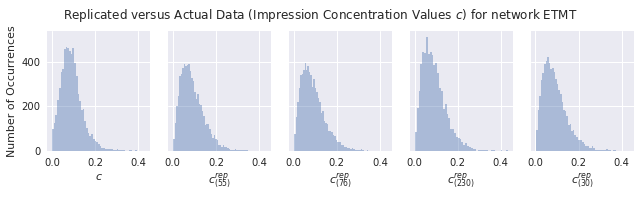
\includegraphics[scale=0.35]{ETMT_c_rep}
      \end{subfigure}
      \begin{subfigure}[b]{.75\textwidth}
        \centering
        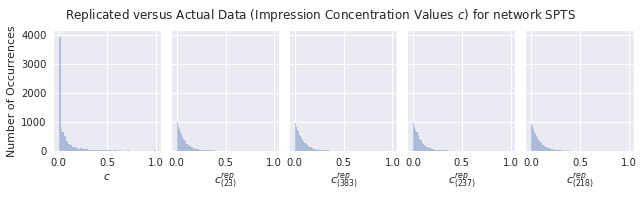
\includegraphics[scale=0.35]{SPTS_c_rep}
      \end{subfigure}
    \end{figure}
\end{frame}

\begin{frame}
\frametitle{Test Statistics}
\begin{itemize}
\item We can quantify model discrepancies by defining a test quantity $T(y, \theta)$
    and then measuring the discrepancy between the observed data and the replicated data.
\pause
\item Formally, we can compute a posterior predictive $p$-value defined as
\begin{align*}
  p_B = \text{Pr}\left( T(y^{\text{rep}}, \theta) \geq T(y, \theta)  | y \right).
\end{align*}
\pause
\item Since we use simulated values of the posterior density, we have that the estimated
$p$-value for $S$ simulations is given by:
\begin{align}
  \hat{p_B} = \frac{1}{S}\sum_{i=1}^S [T(y_{(i)}^{\text{rep}}, \theta_{(i)}) \geq T(y, \theta_{(i)})].
\end{align}

\end{itemize}
\end{frame}

\begin{frame}
\frametitle{Test Statistics - Definition}
We define the following test quantities to use in evaluating the fit of model $\mathcal{M}$:
\begin{itemize}
\item $T_1(y, \theta):= \min(y)$,
\pause
\item $T_2(y, \theta):= \overline{y} = \frac{1}{N}\sum_{i=1}^N y_i$,
\pause
\item $T_3(y, \theta):= \max(y)$,
\pause
\item $T_4(y, \theta):= \text{std}(y) = \sqrt {\frac {\sum _{i=1}^{N}(y_{i}- \overline {y})^{2}}{N-1}}$.
\end{itemize}
\end{frame}

\begin{frame}
  \frametitle{Test Statistics - Evaluation - BCST network}
  \centering
      \begin{tabular}{lrcccccccc}
        Test quantity & $T(y, \theta)$ & \pbox{2cm}{95\% int. for $T(y^{\text{rep}}, \theta)$} & $p_B$ \\ \\
        \hline \\
        $T_1(y, \theta)$ (min) & 3701 & [6245, 14270] & 0.99 \\
        $T_2(y, \theta)$ (mean) & 227457.84 & [2266852.49, 236367.09] & 0.95 \\
        $T_3(y, \theta)$ (max) & 4311038 & [3443885, 4989241] & 0.34 \\
        $T_4(y, \theta)$ (std) & 334052.86 & [325128.37, 364859.10] & 0.90
      \end{tabular}
\end{frame}

\begin{frame}
  \frametitle{Test Statistics - Evaluation - ETMT network}
  \centering
      \begin{tabular}{lrcc}
        Test quantity & $T(y, \theta)$ & \pbox{2cm}{95\% int. for $T(y^{\text{rep}}, \theta)$} & $p_B$ \\ \\
        \hline \\
        $T_1(y, \theta)$ (min) & 0 & [9, 182] & 1.0 \\
        $T_2(y, \theta)$ (mean) & 16357.80 & [16705.39, 17489.11] & 1.0 \\
        $T_3(y, \theta)$ (max) & 452762 & [307901, 760822] & 0.78  \\
        $T_4(y, \theta)$ (std) & 17686.89 & [20021.24, 23205.09] & 1.0
      \end{tabular}
\end{frame}

\begin{frame}
  \frametitle{Test Statistics - Evaluation - SPTS network}
  \centering
  \begin{tabular}{lrcc}
    Test quantity & $T(y, \theta)$ & \pbox{2cm}{95\% int. for $T(y^{\text{rep}}, \theta)$} & $p_B$\\ \\
    \hline \\
    $T_1(y, \theta)$ (min) & 0 & [0, 0] & 1.0 \\
    $T_2(y, \theta)$ (mean) & 3972.45 & [3714.91, 4559.66] & 0.73 \\
    $T_3(y, \theta)$ (max) & 526816 & [607186, 2239365] & 0.99 \\
    $T_4(y, \theta)$ (std) & 22300.18 & [20012.59, 39808.44] & 0.88
  \end{tabular}

\end{frame}

\begin{frame}
\frametitle{Residual Analysis}
\begin{itemize}
    \item For a model with unknown parameters $\theta$ and predictors $x_i$, the \emph{predicted}
    value is $\text{E}(y_i | x_i, \theta)$ and the \emph{residual} is $r_i = y_i - \text{E}(y_i | x_i, \theta)$.
    \pause
    \item The \emph{standardized residual} is given by $r_i / \text{std}(y)$.
    \pause
    \item Using the simulated posterior density, we can compute $\text{E}(y_i | x_i, \theta)$
    to be the mean of the replicated hold-out data itself.
\end{itemize}
\end{frame}

\begin{frame}
\frametitle{Residual Analysis - Actual versus Replicated}
    \begin{figure}[!h]
      \begin{subfigure}[b]{.75\textwidth}
        \centering
        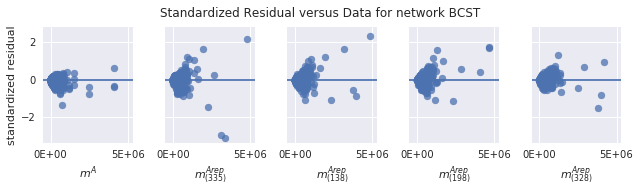
\includegraphics[scale=0.33]{BCST_res}
      \end{subfigure}
      \begin{subfigure}[b]{.75\textwidth}
        \centering
        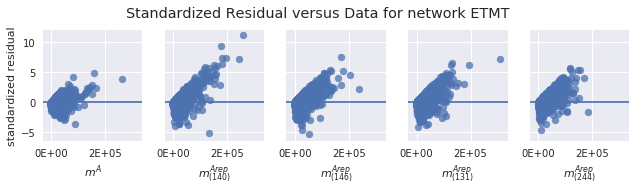
\includegraphics[scale=0.33]{ETMT_res}
      \end{subfigure}
      \begin{subfigure}[b]{.75\textwidth}
        \centering
        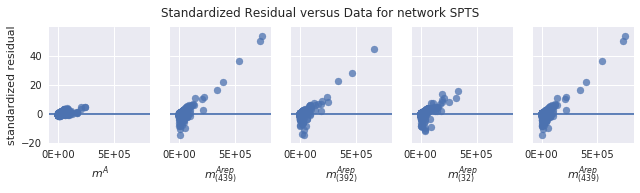
\includegraphics[scale=0.33]{SPTS_res}
      \end{subfigure}
    \end{figure}
\end{frame}


\begin{frame}
\frametitle{Residual Analysis - Test Statistic Evaluation}
    We can measure the residual mis-fit through the following test statistic:
    \begin{align*}
      T(y, \theta, x) = \frac{\overline{r}}{\text{std}(y)}.
    \end{align*}
    \pause
    \begin{figure}[!h]
      \begin{subfigure}[b]{.32\textwidth}
        \centering
        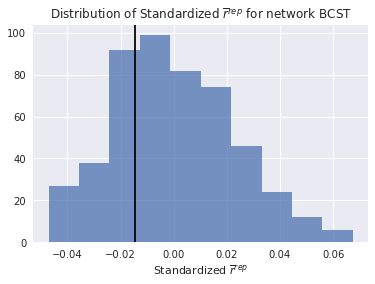
\includegraphics[scale=0.3]{BCST_res_test}
      \end{subfigure}
      \begin{subfigure}[b]{.32\textwidth}
        \centering
        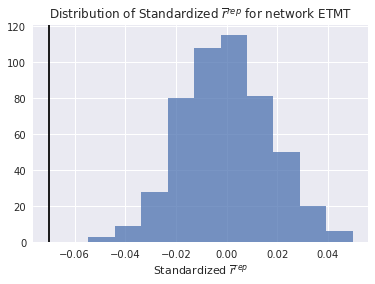
\includegraphics[scale=0.3]{ETMT_res_test}
      \end{subfigure}
      \begin{subfigure}[b]{.32\textwidth}
        \centering
        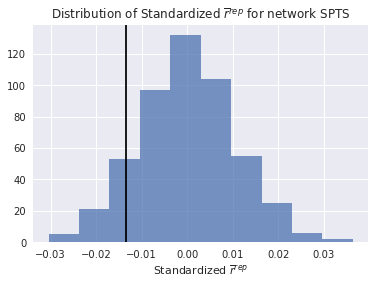
\includegraphics[scale=0.3]{SPTS_res_test}
      \end{subfigure}
    \end{figure}
\end{frame}
\section{Results}

\begin{frame}
\frametitle{Units of Observation}
\end{frame}

\begin{frame}
\frametitle{Quantiled Media Plans}
\end{frame}


\section{Conclusion}

\begin{frame}
\frametitle{Sample frame title}
\end{frame}


\end{document}